\documentclass{beamer}
\usepackage{hyperref}
\usepackage{xcolor}
\usepackage{graphicx}
\usepackage{tikz}
\usetikzlibrary{positioning}
\usepackage{authoraftertitle}
\usepackage{fontspec}

% Define a custom command called \OswaldFont
\newfontfamily\OswaldFont{Oswald}[
    Path=./OswaldFontFiles/,
    Scale=0.9,
    Extension=.ttf,
    UprightFont=*-Regular,
    BoldFont=*-Bold
]
% \setsansfont{Oswald}[Path=./OswaldFontFiles/,Scale=0.9,Extension=.ttf,UprightFont=*-Regular,BoldFont=*-Bold]
    
% \setromanfont{Lato}[Path=./LatoFontFiles/,Scale=0.9,Extension=.ttf,UprightFont=*-Regular,BoldFont=*-Bold]    

\setbeamertemplate{navigation symbols}{}

\title{Zero-Knowledge Protocols }
\newcommand\Facultate{Faculty of Mathematics and Computer Science}
\newcommand\Universitate{Babe\c{s}-Bolyai University}
\newcommand\Adresa{1 Mihail Kog\u{a}lniceanu Street\\ Cluj-Napoca, Cluj, Rom\^{a}nia}
\newcommand\Website{www.cs.ubbcluj.ro}
\newcommand\DataPrezentarii{15/01/2026}

\usepackage{CSTheme_EN}

\begin{document}
%GTITLE PAGE
%custom/title.tex
% Title slide frame
\begin{frame}[plain]
\begin{tikzpicture}[remember picture,overlay]
% Background image
\node[above right,inner sep=0pt] at (current page.south west)
{
    
\includegraphics[width=\paperwidth]{img/blueCS_background.png}
};
    
% Title & Subtitle

\node[above=1.5cm,color=yellowCS,align=center] (title) at (current page.center)
{
    \Huge \MyTitle
};

% Author 
\node[color=white,below=0.1cm] (author) at (title.south){\MyAuthor};
% Facultate
\node[color=yellowCS,below=1cm] (date) at (author.south){\large \Facultate};
% Universitate
\node[color=white,below=1.5cm] (date) at (author.south){\large \Universitate};
% Logo CS
\node[below right=3.5cm and 0.5cm] at (current page.north west)
{
    \includegraphics[width=2cm]{img/CS_white_logo.png}
};
\draw[yellowCS, ultra thick] (3,-0.65) -- (8,-0.65);
% Logo UBB
\node[below right =3.5cm and 10cm] at (current page.north west)
{
    \includegraphics[width=2cm]{img/Sigla_UBB_claudiopolitana_alb.png}
};
\end{tikzpicture}
    
\end{frame}



%CONTINUT EFECTIV SLIDE-URI
% [t] moves everything to the top
\begin{frame}[t] 
    % \Huge makes the title text much bigger
    \frametitle{\Huge Content} 

    \vspace{0.2cm} % Optional: Adds a tiny breather space after the big title

    \begin{columns}[T]
        % LEFT COLUMN
        \begin{column}{0.6\textwidth}
            % This pulls the list closer to the left edge
            \setlength{\leftmargini}{15pt} 
            
            \setbeamertemplate{enumerate item}{\color{blueCS}\insertenumlabel.}
            \setlength{\itemsep}{0.6em} % Increases space between items for readability
            
            \begin{enumerate}
                \item Introduction: The Privacy Dilemma
                \item Definition and Actors
                \item Brief History
                \item Core Properties
                \item Interactive vs. Non-Interactive ZKPs
                \item zk-SNARKs
                \item zk-STARKs
                \item Bulletproofs
                \item Trade-Offs & Comparison
                \item Real-World Applications
                \item Conclusions
            \end{enumerate}
        \end{column}

        % RIGHT COLUMN (The Image)
        \begin{column}{0.4\textwidth}
             \centering
             % Ensure you have the image file in your folder
             % \includegraphics[width=\textwidth]{img/diagram.png}
        \end{column}
    \end{columns}
\end{frame}

% SLIDE 3: INTRODUCTION
\begin{frame}{Introduction: The Privacy Dilemma}

    % Use small font size to ensure text fits
    \small 

    % TOP SECTION: Text Content
    \begin{columns}[T]
        \begin{column}{0.95\textwidth}
            \begin{itemize}
                % Reduce spacing between main items (was 0.8em)
                \setlength\itemsep{0.4em} 
                
                \item \textbf{The Fundamental Conflict} 
                \newline To verify a claim, we typically demand access to the underlying data (Privacy vs. Verification).
                
                \item \textbf{The Standard Model (``Trivial Proofs'')} 
                \newline To verify data, we usually have to reveal it.
                \begin{itemize}
                    \setlength\itemsep{0.2em} % Tighter spacing for sub-items
                    % \item \textit{Example:} Showing an ID card to prove age reveals your address.
                    % \item \textit{Flaw:} This creates massive data leaks and honeypots.
                \end{itemize}
                
                \item \textbf{The Zero-Knowledge Goal} 
                \newline Proving a statement is true \textbf{without} conveying any information apart from the fact that it is true.
            \end{itemize}
        \end{column}
    \end{columns}

    \vfill % Push the diagram to the bottom

    % --- DIAGRAM SECTION ---
    % scaling down slightly and centering
    \begin{figure}[h]
        \centering
        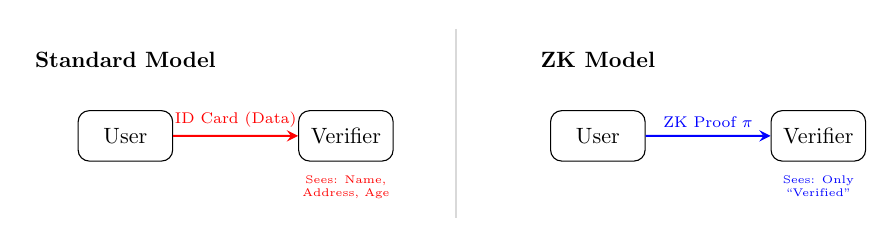
\begin{tikzpicture}[
            scale=0.8, transform shape, 
            box/.style={draw, rectangle, rounded corners, minimum height=0.8cm, minimum width=1.5cm, align=center, fill=white},
            arrow/.style={->, thick, >=stealth}
        ]
            % --- LEFT SIDE: STANDARD MODEL ---
            \node[font=\bfseries] (std_title) at (0,0) {Standard Model};
            \node[box] (user1) at (0, -1.2) {User};
            \node[box] (ver1) at (3.5, -1.2) {Verifier};
            
            % Red Arrow for Standard Model
            \draw[arrow, red] (user1) -- node[above, font=\scriptsize, text=red] {ID Card (Data)} (ver1);
            \node[below=0.1cm of ver1, font=\tiny, text=red, align=center] {Sees: Name,\\Address, Age};

            % --- DIVIDER LINE (Vertical) ---
            \draw[thick, gray!30] (5.25, 0.5) -- (5.25, -2.5);

            % --- RIGHT SIDE: ZK MODEL ---
            \node[font=\bfseries] (zk_title) at (7.5,0) {ZK Model};
            \node[box] (user2) at (7.5, -1.2) {User};
            \node[box] (ver2) at (11.0, -1.2) {Verifier};
            
            % Blue Arrow for ZK Model
            \draw[arrow, blue] (user2) -- node[above, font=\scriptsize, text=blue] {ZK Proof $\pi$} (ver2);
            \node[below=0.1cm of ver2, font=\tiny, text=blue, align=center] {Sees: Only\\``Verified''};

        \end{tikzpicture}
    \end{figure}
    \vspace{0.1cm} % Small bottom padding
\end{frame}

% SLIDE 4a: DEFINITION (Text Focus)
\begin{frame}{Definition \& The Core Actors}

    % 1. Formal Definition
    \begin{block}{Formal Definition}
        A \textbf{Zero-Knowledge Protocol} is a method by which one party (the Prover) can prove to another party (the Verifier) that a given statement is true, without conveying any additional information apart from the fact that the statement is indeed true.
    \end{block}

    \vspace{0.5cm}

    % 2. The Actors
    \begin{itemize}
        \setlength\itemsep{0.8em} % Comfortable spacing
        \item \textbf{The Prover ($P$):} An entity with unlimited computational power (theoretically) who holds a secret \textit{witness} ($w$).
        \item \textbf{The Verifier ($V$):} An entity with bounded computational power who validates the proof. $V$ must not learn $w$.
        \item \textbf{The Witness ($w$):} The secret input (e.g., a password, a private key) that certifies the statement.
    \end{itemize}

\end{frame}


% SLIDE: BRIEF HISTORY
\begin{frame}{Brief History of ZKPs}

    \small 
    
    % Pull text up slightly to make room for bottom figure
    \vspace*{-0.5cm}

    \begin{itemize}
        \setlength\itemsep{0.3em} % Tighter spacing
        
        \item \textbf{1985: The Theoretical Birth}
        \newline Shafi Goldwasser, Silvio Micali, and Charles Rackoff published the fundamental paper defining zero-knowledge for the first time.
        
        \item \textbf{2010s: From Theory to Practice}
        \newline For decades, ZKPs were theoretical. In 2012, new protocols (like Pinocchio) made it possible to generate proofs fast enough for real computers.
        
        \item \textbf{2016: The Blockchain Era}
        \newline The launch of \textbf{Zcash}, the first cryptocurrency to implement zk-SNARKs, proving private transactions were possible at scale.
    \end{itemize}

    \vspace{0.2cm}

    \begin{center}
        % Scale reduced to 0.8 to prevent cut-off
        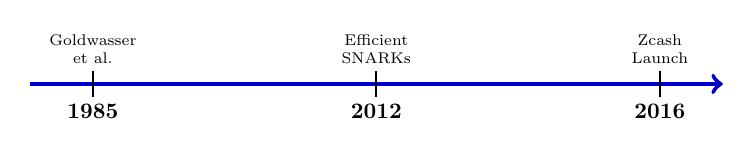
\begin{tikzpicture}[scale=0.8, transform shape]
            % Main Line
            \draw[->, ultra thick, blue!80!black] (0,0) -- (11,0);

            % 1985 Tick
            \draw[thick] (1, 0.2) -- (1, -0.2);
            \node[below=0.2cm, font=\bfseries] at (1,0) {1985};
            \node[above=0.2cm, align=center, font=\scriptsize] at (1,0) {Goldwasser\\et al.};

            % 2012 Tick
            \draw[thick] (5.5, 0.2) -- (5.5, -0.2);
            \node[below=0.2cm, font=\bfseries] at (5.5,0) {2012};
            \node[above=0.2cm, align=center, font=\scriptsize] at (5.5,0) {Efficient\\SNARKs};

            % 2016 Tick
            \draw[thick] (10, 0.2) -- (10, -0.2);
            \node[below=0.2cm, font=\bfseries] at (10,0) {2016};
            \node[above=0.2cm, align=center, font=\scriptsize] at (10,0) {Zcash\\Launch};
        \end{tikzpicture}
    \end{center}

\end{frame}

% SLIDE 6: CORE PROPERTIES
\begin{frame}{The Three Core Properties}

    \small

    For a protocol to be considered "Zero-Knowledge," it must strictly satisfy these three conditions:

    \vspace{0.3cm}

    \begin{enumerate}
        \setlength\itemsep{0.8em}
        
        \item \textbf{1. Completeness} (Reliability)
        \newline If the statement is true and the Prover is honest, the Verifier will \textbf{always} be convinced.
        \newline \textit{($P(\text{Verifier accepts} \mid \text{True}) = 1$)}

        \item \textbf{2. Soundness} (Security)
        \newline If the statement is false, a cheating Prover cannot convince the Verifier, except with a negligible probability.
        \newline \textit{($P(\text{Verifier accepts} \mid \text{False}) \approx 0$)}

        \item \textbf{3. Zero-Knowledge} (Privacy)
        \newline If the statement is true, the Verifier learns nothing other than the fact that the statement is true. They cannot reverse-engineer the secret witness $w$ from the proof.
    \end{enumerate}

    \vspace{0.5cm}
    
    \begin{center}
        \textbf{In simple terms:} "It works, you can't cheat, and you don't leak secrets."
    \end{center}

\end{frame}

% SLIDE 7a: INTERACTIVE ZKP
\begin{frame}{Interactive ZKPs (1/2)}

    \small

    \begin{itemize}
        \item \textbf{Mechanism:} The Prover and Verifier must be online simultaneously and exchange multiple messages.
        \item \textbf{The 3-Step "Sigma Protocol":}
        \begin{enumerate}
            \item \textbf{Commitment ($t$):} Prover sends a temporary value to "lock" their secret.
            \item \textbf{Challenge ($c$):} Verifier picks a random question.
            \item \textbf{Response ($s$):} Prover answers using the secret and the random challenge.
        \end{enumerate}
        \item \textbf{Limitation:} Not scalable for blockchains (you can't have every miner challenge every transaction sender).
    \end{itemize}

    \vspace{0.3cm}

    % INTERACTIVE DIAGRAM (Safe Mode)
    \begin{center}
        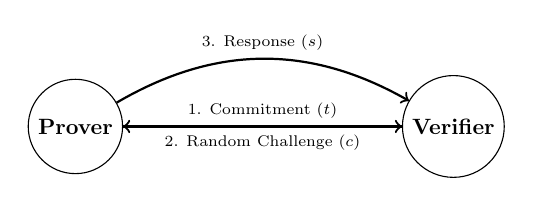
\begin{tikzpicture}[scale=0.8, transform shape]
            % Actors
            \node[draw, circle, font=\bfseries] (P) at (0,0) {Prover};
            \node[draw, circle, font=\bfseries] (V) at (6,0) {Verifier};

            % Arrows
            \draw[->, thick] (P) -- node[above, font=\scriptsize] {1. Commitment ($t$)} (V);
            \draw[<-, thick] (P) -- node[below, font=\scriptsize] {2. Random Challenge ($c$)} (V);
            \draw[->, thick] (P) to[bend left=30] node[above, font=\scriptsize] {3. Response ($s$)} (V);
        \end{tikzpicture}
    \end{center}

\end{frame}


% SLIDE 7b: NON-INTERACTIVE ZKP
\begin{frame}{Non-Interactive ZKPs (2/2)}

    \small

    \begin{itemize}
        \item \textbf{Goal:} The Prover generates a single proof string $\pi$ that anyone can verify later. No interaction required.
        \item \textbf{The Solution (Fiat-Shamir Heuristic):} 
        \newline We replace the human Verifier with a cryptographic \textbf{Hash Function}.
        \item \textbf{How it works:}
        \newline Instead of waiting for a random challenge $c$, the Prover calculates:
        $$ c = \text{Hash}(\text{Commitment}, \text{Statement}) $$
        \item \textbf{Result:} The "Challenge" is still random (pseudo-random) and unforgeable, but computed automatically.
    \end{itemize}

    \vspace{0.2cm}

    % NIZK DIAGRAM
    \begin{center}
        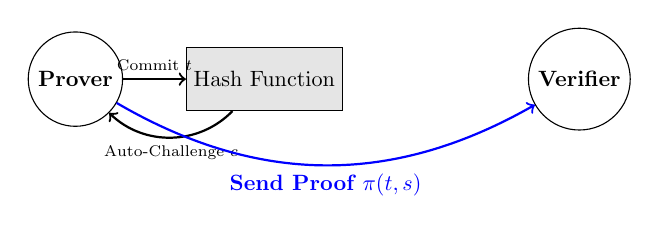
\begin{tikzpicture}[scale=0.8, transform shape]
            % Prover
            \node[draw, circle, font=\bfseries] (P) at (0,0) {Prover};

            % Hash Box (The "Virtual Verifier")
            \node[draw, rectangle, fill=gray!20, minimum height=1cm] (H) at (3,0) {Hash Function};

            % Real Verifier
            \node[draw, circle, font=\bfseries] (V) at (8,0) {Verifier};

            % Arrows
            \draw[->, thick] (P) -- node[above, font=\scriptsize] {Commit $t$} (H);
            \draw[->, thick] (H) to[bend left=45] node[below, font=\scriptsize] {Auto-Challenge $c$} (P);
            \draw[->, thick, blue] (P) to[bend right=30] node[below, font=\bfseries] {Send Proof $\pi(t,s)$} (V);

        \end{tikzpicture}
    \end{center}

\end{frame}


% SLIDE 8: zk-SNARKs (FIXED SPACING)
\begin{frame}{zk-SNARKs: The Industry Standard}

    \small

    \textbf{Zero-Knowledge Succinct Non-Interactive Argument of Knowledge}
    
    % Reduced space here
    \vspace{0.1cm}

    \begin{itemize}
        \setlength\itemsep{0.3em} % Tighter spacing for top list
        \item \textbf{Succinct:} The proof is incredibly small (typically $\approx 288$ bytes) and takes milliseconds to verify, regardless of computation complexity.
        \item \textbf{Argument:} Strictly speaking, it is an "argument" (computationally sound) rather than a "proof" (statistically sound). It relies on cryptographic hardness assumptions.
    \end{itemize}

    % Reduced space here to pull the block up
    \vspace{0.2cm}

    % THE TRUSTED SETUP BLOCK
    \begin{block}{The Achilles' Heel: Trusted Setup}
        SNARKs require an initial generation event to create a \textbf{Common Reference String (CRS)}.
        \begin{itemize}
            \setlength\itemsep{0.3em} % Tighter spacing inside block
            \item The random numbers used to create the CRS are called \textbf{"Toxic Waste."}
            \item \textbf{Risk:} If this waste is not destroyed, the creator can forge fake proofs (breaking Soundness), though they still cannot read secrets.
        \end{itemize}
    \end{block}

\end{frame}

% SLIDE 9: zk-STARKs
\begin{frame}{zk-STARKs: The Post-Quantum Solution}

    \small

    \textbf{Zero-Knowledge Scalable Transparent Argument of Knowledge}

    \vspace{0.2cm}

    \begin{itemize}
        \setlength\itemsep{0.5em}
        \item \textbf{Transparent:} No "Trusted Setup" is required.
        It relies on publicly verifiable randomness, eliminating the "Toxic Waste" risk entirely.
        
        \item \textbf{Post-Quantum Secure:} 
        unlike SNARKs (which rely on Elliptic Curve Cryptography), STARKs rely on hash functions and information theory. They are resistant to attacks from future quantum computers.
        
        \item \textbf{Scalable:} 
         Verification time scales \textit{poly-logarithmically} ($O(\log^2 n)$). As the complexity of the computation ($n$) grows massive, the verification time barely increases.
    \end{itemize}

    \vspace{0.2cm}

    % VISUAL COMPARISON (Safe Mode)
    \begin{center}
        \begin{tikzpicture}[scale=0.8, transform shape]
            % 1. The Trade-off (Proof Size)
            \node[draw, rectangle, rounded corners, fill=red!10, align=center, width=3cm] (Size) at (0,0) {\textbf{The Cost}\\Larger Proofs\\(40kB - 200kB)};

            % 2. The Arrow
            \draw[->, ultra thick, gray] (2.5, 0) -- (5.5, 0);

            % 3. The Benefits (Security)
            \node[draw, rectangle, rounded corners, fill=green!10, align=center, width=3cm] (Sec) at (8,0) {\textbf{The Benefit}\\Quantum Safe\\\& No Toxic Waste};
            
            % Icons/Labels
            \node[below=0.1cm of Size, font=\tiny] {vs SNARKs ($\approx$ 288 bytes)};
            \node[below=0.1cm of Sec, font=\tiny] {Future Proof};

        \end{tikzpicture}
    \end{center}

\end{frame}

% SLIDE 10: Arithmetization (The Trace)
\begin{frame}{Step 1: Arithmetization (Trace to Polynomial)}
    \small
    How to prove we've actually processed some data? (Prover's side)
    
    \vspace{0.2cm}

    \begin{columns}
        % COLUMN 1: The Execution Trace
        \begin{column}{0.45\textwidth}
            \textbf{1. Execution Trace} \\
            \textit{Record it privately}
            \vspace{0.2cm}
            \begin{table}
                \centering
                \begin{tabular}{|c|c|}
                    \hline
                    \textbf{Step} ($i$) & \textbf{Value} ($x_i$) \\
                    \hline
                    0 & 3 \\
                    1 & 9 \\
                    2 & 81 \\
                    3 & 6561 \\
                    \hline
                \end{tabular}
            \end{table}
        \end{column}

        % COLUMN 2: Interpolation
        \begin{column}{0.55\textwidth}
            \textbf{2. Interpolation} \\
            \textit{We find a polynomial $T(x)$ that passes through these points.}
            \vspace{0.3cm}
            
            \[
            T(g^i) = x_i
            \]
            \vspace{0.1cm}
            \begin{itemize}
                \footnotesize
                \item The steps are mapped to a finite field generator $g$.
                \item $T(x)$ captures the \textbf{entire} history of the computation in a single curve.
                \item All this becomes \textbf{the witness}
            \end{itemize}
        \end{column}
    \end{columns}
\end{frame}

% SLIDE 11: Constraints & The Quotient
\begin{frame}{Step 2: The "Honesty" Check}
    \small
    We define a rule (Constraint) that must equal \textbf{Zero} if the computation is valid. This is public
    
    \vspace{0.2cm}

    \begin{block}{1. The Transition Constraint $C(x)$}
        For a rule like $x_{next} = x^2$, the constraint is:
        \[ C(T(x)) = T(g \cdot x) - T(x)^2 = 0 \]
        \textit{(This must be zero at every valid step $g^0, g^1, \dots$)}
    \end{block}

    \vspace{0.2cm}

    \begin{block}{2. The Quotient Polynomial $Q(x)$}
        If the Prover is honest, $C(T(x))$ is perfectly divisible by the \textbf{Vanishing Polynomial} $Z(x)$ (which is zero at all steps).
        
        \[ Q(x) = \frac{C(T(x))}{Z(x)} \]
        
        \begin{itemize}
            \item \textbf{Honest:} $Q(x)$ is a clean, low-degree polynomial.
            \item \textbf{Cheating:} The division fails (remainder) or degree explodes.
        \end{itemize}
    \end{block}
\end{frame}

% SLIDE 12: The Spot Check (Verification)
\begin{frame}{Step 3: The Verification (Soundness)}
    \small
    The Verifier does not check the whole table. They check a random point.
    
    \vspace{0.3cm}

    \textbf{The Protocol:}
    \begin{enumerate}
        \setlength\itemsep{0.6em}
        \item \textbf{Commit:} Prover sends Merkle Root of $T(x)$ and $Q(x)$.
        \item \textbf{Challenge:} Verifier picks a random point $z$ (e.g., $z=42$).
        \item \textbf{Query:} Prover reveals $T(z), T(g \cdot z), Q(z)$.
        \item \textbf{Check:} Verifier runs the equation locally:
    \end{enumerate}

    \vspace{0.2cm}
    
    \begin{center}
        \fcolorbox{black}{yellow!10}{
            \Large $T(g \cdot z) - T(z)^2 \stackrel{?}{=} Q(z) \cdot Z(z)$
        }
    \end{center}

    \vspace{0.3cm}
    \footnotesize
    \textit{*Plus a "Low Degree Test" (FRI) to ensure $T(x)$ isn't just random noise fitting the points.}
\end{frame}

% SLIDE 11: BULLETPROOFS
\begin{frame}{Bulletproofs: The Middle Ground}

    \small

    \textbf{Short Proofs for Confidential Transactions}

    \vspace{0.2cm}

    \begin{itemize}
        \setlength\itemsep{0.5em}
        
        \item \textbf{No Trusted Setup:} 
        \newline Like STARKs, they are transparent. There is no "Toxic Waste" risk.
        
        \item \textbf{The Specialty: Range Proofs} 
        \newline They are mathematically optimized specifically to prove that a secret number lies within a range (e.g., $0 \leq \text{salary} \leq \text{limit}$).
        \newline \textit{This reduces proof size from kilobytes to just $\sim$600 bytes.}

        \item \textbf{The Trade-off:} 
        \newline Verification time is \textbf{linear}. If you try to verify thousands of transactions at once, it is slower than SNARKs/STARKs.
        
        \item \textbf{Adoption:} 
        \newline Used by the cryptocurrency \textbf{Monero} to hide transaction amounts while ensuring no extra coins are created out of thin air.
    \end{itemize}

\end{frame}

% SLIDE 11a: TRADE-OFFS TABLE
\begin{frame}{Trade-Offs Comparison}

    \renewcommand{\arraystretch}{1.5} % Add vertical breathing room in table

    \begin{center}
        % Resize the table to fit the text width
        \resizebox{\textwidth}{!}{%
        \begin{tabular}{|l|c|c|c|c|}
            \hline
            \textbf{Protocol} & \textbf{Proof Size} & \textbf{Verify Speed} & \textbf{Trusted Setup?} & \textbf{Post-Quantum?} \\
            \hline
            
            % SNARKS ROW
            \textbf{zk-SNARKs} & 
            \textcolor{green!60!black}{\textbf{Tiny}} & 
            \textcolor{green!60!black}{\textbf{Fast}} & 
            \textcolor{red}{\textbf{Yes (Risk)}} & 
            \textcolor{red}{No} \\
            & {\scriptsize ($\sim$288 B)} & {\scriptsize ($\sim$10ms)} & & \\
            \hline

            % STARKS ROW
            \textbf{zk-STARKs} & 
            \textcolor{red}{\textbf{Large}} & 
            \textcolor{green!60!black}{\textbf{Fast}} & 
            \textcolor{green!60!black}{\textbf{No}} & 
            \textcolor{green!60!black}{\textbf{Yes}} \\
             & {\scriptsize (45-200 kB)} & {\scriptsize ($\sim$50ms)} & & \\
            \hline

            % BULLETPROOFS ROW
            \textbf{Bulletproofs} & 
            \textcolor{green!60!black}{\textbf{Small}} & 
            \textcolor{red}{\textbf{Slow}} & 
            \textcolor{green!60!black}{\textbf{No}} & 
            \textcolor{red}{No} \\
             & {\scriptsize ($\sim$600 B)} & {\scriptsize (Linear time)} & & \\
            \hline
        \end{tabular}%
        }
    \end{center}

\end{frame}

% SLIDE 11b: SUMMARY OF THE TRILEMMA
\begin{frame}{Summary of the Trilemma}

    \begin{block}{Choosing the Right Protocol}
        There is no "perfect" protocol yet. The choice depends on the specific application requirements:
        
        \vspace{0.3cm}
        
        \begin{itemize}
            \setlength\itemsep{0.6em}
            \item Choose \textbf{zk-SNARKs} for blockchains where on-chain storage cost is expensive (e.g., Ethereum L1).
            \item Choose \textbf{zk-STARKs} for high-integrity systems where "Toxic Waste" is unacceptable and post-quantum security is required.
            \item Choose \textbf{Bulletproofs} for simple range proofs where verification speed is less critical but no trusted setup is desired.
        \end{itemize}
    \end{block}

\end{frame}

% SLIDE 13: REAL-WORLD APPLICATIONS (ING, StarkWare, EY) - NO DIAGRAM
\begin{frame}{Real-World Applications}

    \footnotesize % Smaller font to fit the template margins

    \begin{itemize}
        \setlength\itemsep{1.2em} % More breathing room between items
        
        \item \textbf{1. Enterprise Adoption (ING Bank)}
        \newline Major banks like \textbf{ING} have launched \textbf{Zero-Knowledge Range Proofs}.
        \newline \textit{Use Case:} A client can prove their salary is within a required range for a mortgage without revealing the exact number.

        \item \textbf{2. Scalability with zk-STARKs (StarkWare)}
        \newline \textbf{StarkWare} uses STARKs to power platforms like \textbf{dYdX} (trading) and \textbf{Immutable X} (gaming).
        \newline \textit{Benefit:} They process millions of transactions off-chain and verify them with a single \textbf{post-quantum secure} STARK proof.

        \item \textbf{3. Enterprise Privacy on Public Chains (EY)}
        \newline \textbf{EY} (Ernst \& Young) developed \textbf{Nightfall}, a solution for private business transactions on the public Ethereum network.
        \newline \textit{Technology:} Uses \textbf{zk-SNARKs} to encrypt transaction data while ensuring the transaction is valid.
    \end{itemize}

\end{frame}
% SLIDE 14: CONCLUSIONS (FIXED)
\begin{frame}{Conclusions}

    \small 

    \begin{itemize}
        \setlength\itemsep{0.5em} % Tighter spacing is key here
        \item \textbf{A Paradigm Shift:} 
        \newline We move from \textit{"Trust me, I saw the data"} to \textit{"Verify this math, the data is irrelevant."}
        
        \item \textbf{Solving the Conflict:} 
        \newline ZKPs resolve the tension between \textbf{Privacy} and \textbf{Transparency}.
        
        \item \textbf{The Future:} 
        \newline Hardware acceleration and algorithmic improvements are making ZKPs the standard for the decentralized web.
    \end{itemize}

    \vspace{0.5cm}

    % Final Takeaway Block
    \begin{block}{Final Thought}
        \centering
        \textit{"Zero-Knowledge Proofs allow us to trust the validity of computation without trusting the entity performing it."}
    \end{block}

\end{frame}


% SLIDE 15: REFERENCES (UPDATED WITH CORRECT ING WHITEPAPER)
\begin{frame}{References}

    \tiny % Smallest available font size to fit everything
    \setlength{\itemsep}{0pt} % Remove extra space between items

    \begin{thebibliography}{99}
        
        % 1. The Origin
        \bibitem{GMR85}
        S. Goldwasser, S. Micali, and C. Rackoff.
        \newblock \textit{The Knowledge Complexity of Interactive Proof Systems}.
        \newblock SIAM Journal on Computing, 18(1):186–208, 1989.

        % 2. Fiat-Shamir
        \bibitem{FS86}
        A. Fiat and A. Shamir.
        \newblock \textit{How to Prove Yourself: Practical Solutions to Identification and Signature Problems}.
        \newblock CRYPTO 1986.

        % 3. SNARKs (Zcash)
        \bibitem{Sass14}
        E. Ben-Sasson et al.
        \newblock \textit{Zerocash: Decentralized Anonymous Payments from Bitcoin}.
        \newblock IEEE S\&P 2014.

        % 4. STARKs
        \bibitem{Stark18}
        E. Ben-Sasson, I. Bentov, Y. Horesh, and M. Riabzev.
        \newblock \textit{Scalable, Transparent, and Post-Quantum Secure Computational Integrity}.
        \newblock IACR Cryptology ePrint Archive, 2018.

        % 5. Bulletproofs
        \bibitem{Bunz18}
        B. Bünz et al.
        \newblock \textit{Bulletproofs: Short Proofs for Confidential Transactions and More}.
        \newblock IEEE S\&P 2018.

        % 6. ING Bank (CORRECTED - Sourced from your PDF)
        \bibitem{ING17}
        T. Koens, C. Ramaekers, and C. van Wijk.
        \newblock \textit{Efficient Zero-Knowledge Range Proofs in Ethereum}.
        \newblock ING Bank Whitepaper, 2017.

        % 7. EY Nightfall
        \bibitem{EY25}
        EY Global.
        \newblock \textit{EY upgrades Nightfall: A zero-knowledge roll-up enabling private transactions on the Ethereum blockchain}.
        \newblock EY Newsroom, April 2025.

    \end{thebibliography}

\end{frame}

% SLIDE 16: Q&A / THANK YOU
\begin{frame}
    \centering
    \vspace{1cm}
    
    {\Huge \textbf{Thank You!}}
    
    \vspace{1cm}
    
    
    \vspace{1.5cm}
    
    \footnotesize
    \Facultate \\
    \Universitate
    
\end{frame}


\end{document}
